\documentclass[12pt]{article}
\usepackage[utf8]{inputenc}
\usepackage{graphicx}
\usepackage[a4paper, total={6in, 8in}]{geometry}
\usepackage{listings}
\usepackage{color}
\graphicspath{ {images/} }
 
\title{Lab work report 9 - Norm}
\author{Cao Anh Quan - ICT Master}
\date{November 13, 2016}
 
 
\begin{document}
 
\begin{titlepage}
\maketitle
\end{titlepage}

The employee database satisfy the 3NF because:

\begin{itemize}
\item There is no repeated column
\item Cell contains only atomic
\item Each non-key column depends on the primary key
\item The columns in table depend on the primary key
\end{itemize}

There are 3 main Concepts: Customer, Order, Product. 1 Customer may have many Order and 1 Order can only belong to one Customer. 1 Product can belong to many Order and vice versa, thus we need to have one more intermediate table ProductOrder.

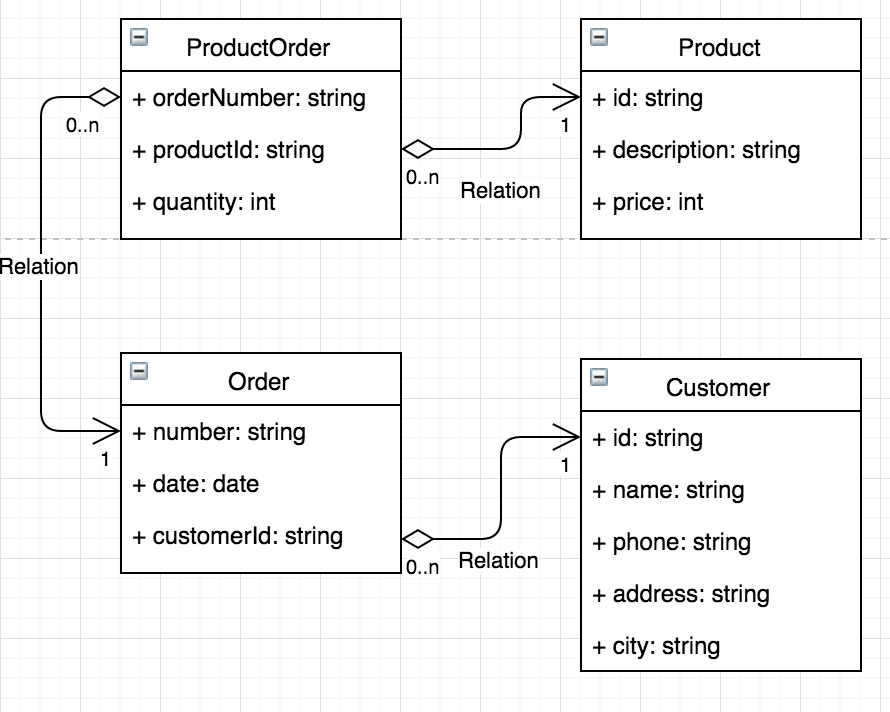
\includegraphics[width=\textwidth]{order.png}

 
\end{document}
